\Transcb{yellow}{blue}{Observation of high-energy photons}
\vspace*{1cm}
\begin{center}
{\blue Compton Gamma Ray Observatory}\\[5mm]
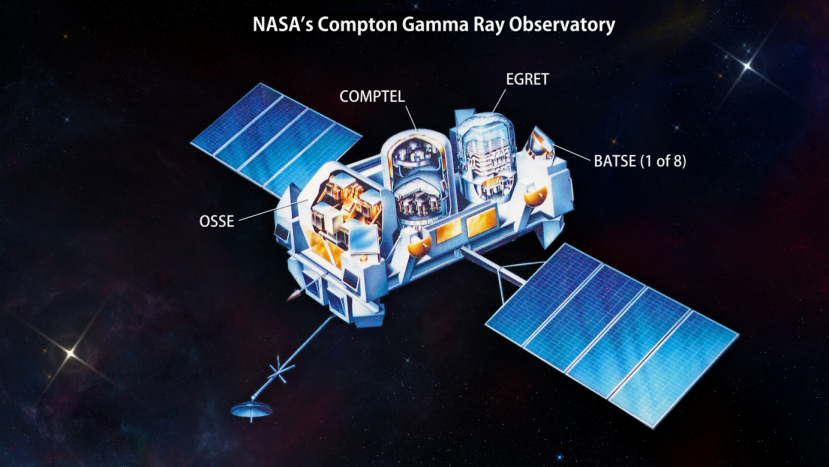
\includegraphics[keepaspectratio,width=13.5cm]{cgro2}
\end{center}

\newpage
\vspace*{2mm}
%
\begin{itemize}
\item COMPTEL (sky maps, spectroscopy)
\item[] Compton Telescope
\item[] Wide field 1-30 MeV
{\blue
\item EGRET (AGN, GRBs, Pulsars)
\item[] Energetic Gamma Ray Exp. Telescope
\item[] Wide field 20 MeV - 30 GeV
}
\item OSSE (X-ray sources, QSO spectra, SNe)
\item[] Oscillating Scintillation Spectrometer Exp.
\item[] Narrow field ($4^{0} \times 11^{0}$) 50 keV - 10 MeV
{\blue
\item BATSE (All sky monitor, GRBs)
\item[] Burst and Transient Source Experiment
\item[] Wide field (8 elements) 20 keV - 30 MeV
}
\end{itemize}

\Tr
\vspace*{0.5cm}
\begin{center}
{\blue The WHIPPLE gamma ray telescope}\\[5mm]
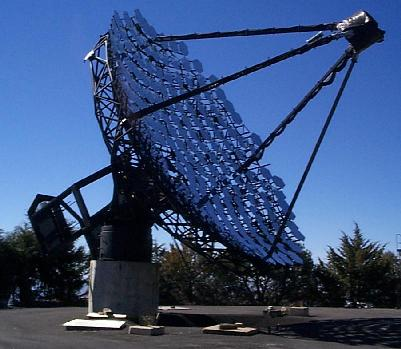
\includegraphics[keepaspectratio,width=12cm]{whipple}
\end{center}

\newpage
\vspace*{3cm}
%
\begin{itemize}
\item Ground based (Arizona, USA)
\item[] Reflective 10 meter diameter dish
\item Cerenkov radiation from air showers
\item[] Field of view : $3^{0}$
\item[] Shower energy 100 GeV - 10 TeV
\end{itemize}

\Tr
\onecolumn
\begin{center}
{\blue Observations of Markarian 421}
\end{center}
%
\begin{itemize}
\item Markarian 421 : AGN at a distance of about 100 Mpc ($z=0.031$).
\item Discovered in 1991 by TeV gamma rays (Nature 160 (1992) 477).
\item Observed by EGRET (1991-1993) and Whipple 1993-1994 : Flare at 14-15 may 1994.
\item[] (ApJ 438 (1995) L59. $\quad$  ApJS 94 (1994) 551.)
\item EGRET ($E_{\gamma}>100$~MeV) : constant flux of $(1.7 \pm 0.3) \cdot 10^{-7}$ photons cm$^{-2}$ s$^{-1}$ 
\item Whipple ($E_{\gamma}>250$~GeV) : average flux of $(2.3 \pm 0.3) \cdot 10^{-11}$ photons cm$^{-2}$ s$^{-1}$ 
\item[] Flux during 1994 flare : $(2.1 \pm 0.3) \cdot 10^{-10}$ photons cm$^{-2}$ s$^{-1}$ 
\end{itemize}

\begin{center}
\colorbox{yellow}{Can the fireball model be probed ?}\\[5mm]
in other words :\\[5mm]
\colorbox{yellow}{Can we indicate hadronic processes in these objects ?}
\end{center}
%
Even more violent transient phenomena are observed ...
\Tr
\twocolumn
\begin{center}
{\blue Batse GRB trigger 109}\\[5mm]
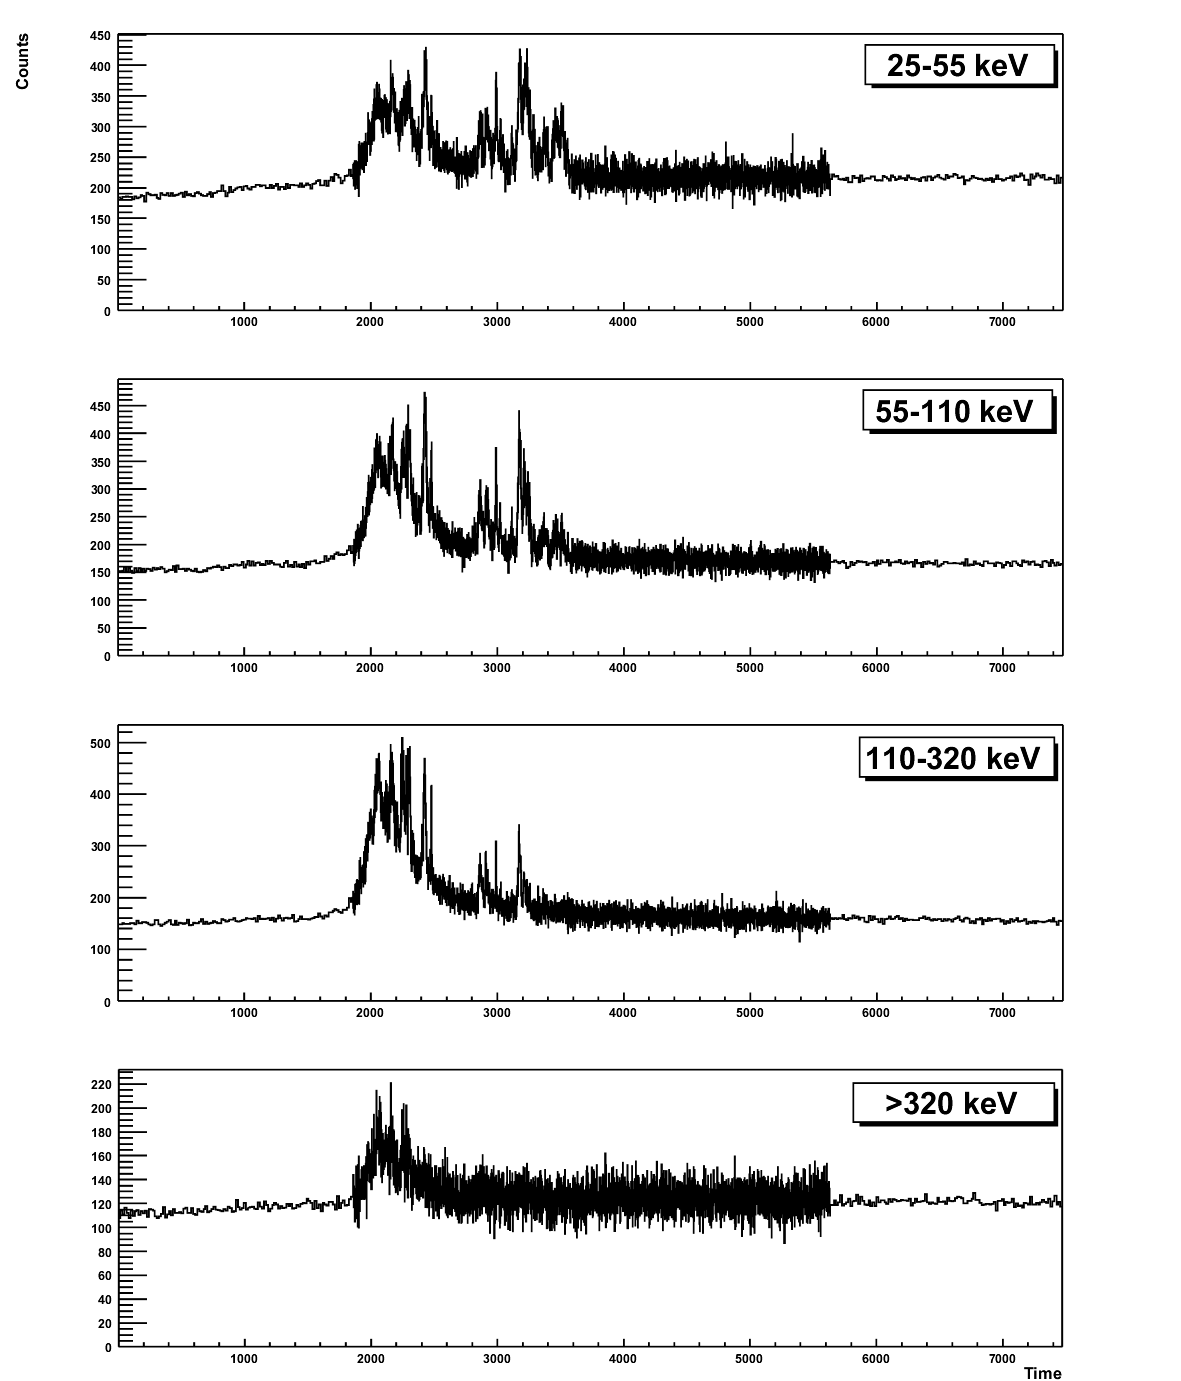
\includegraphics[keepaspectratio,height=14cm]{batse-109}
\end{center}

\newpage

\vspace*{2cm}
%
\begin{itemize}
\item Burst lasts $\sim$2 minutes
\item Rich (energy dependent ?) structure
\begin{itemize}
\item Rather compact source involved
\item Process might consist of several phases
\item[] Various shock waves ?
\end{itemize}
\item[] What are these GRBs ?
\begin{itemize}
\item Common features ?
\item Where are they located ?
\end{itemize}
\end{itemize}

\Tr
\twocolumn[\begin{center}{\blue Burst duration analysis}\end{center}]
%
\vspace*{0.5cm}
%
\begin{center}
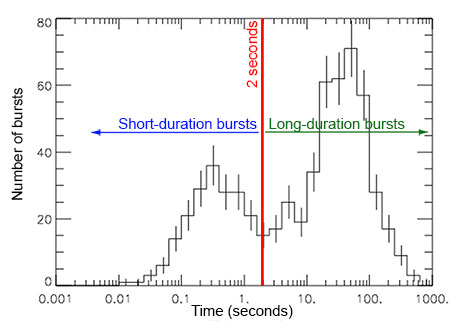
\includegraphics[keepaspectratio,width=13cm]{GRB-T90}
\end{center}

\newpage

\vspace*{1cm}
%
\begin{itemize}
\item t90 $\equiv \Delta t$ from 5\% to 95\% of fluence
\item Two classes : short and long bursts ?
\begin{itemize}
\item Long : dense medium (hypernovae ?)
\item Short : dilute medium (mergers ?)
\end{itemize}
\item[] {\blue Effect of (cosmological) time dilation ?}
\end{itemize}

\Tr
\onecolumn
\begin{center}
{\blue Possible GRB scenarios}\\[3mm]
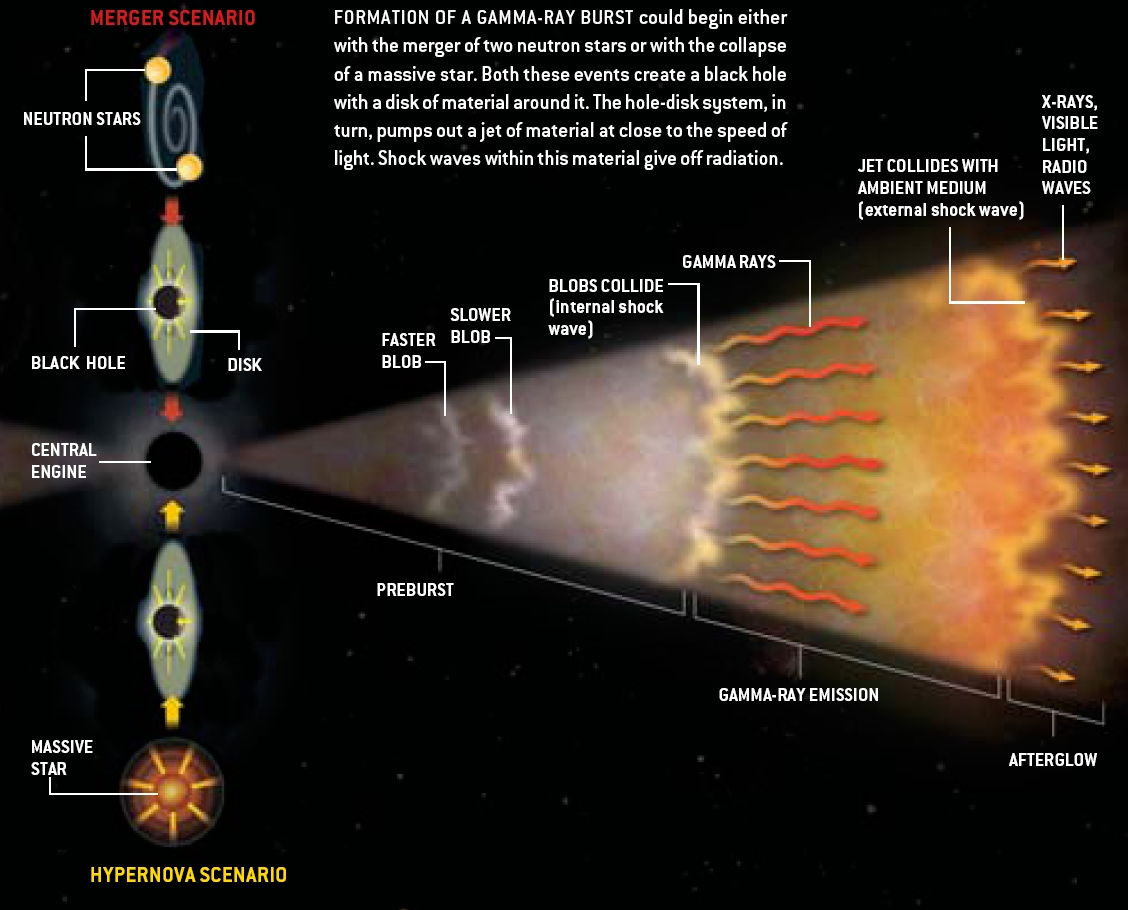
\includegraphics[keepaspectratio,height=13.5cm]{GRB-phases2}\\[2mm]
{\red Multi-Messenger studies may provide insight in the various processes} 
\end{center}

\Tr
\twocolumn
\begin{itemize}
\item GW170817: a NS-NS merger
\item[] $M_{1} \approx 1.2M_{\odot} \quad M_{2} \approx 1.5M_{\odot}$
\item[] $D \approx 40$ Mpc
\item Weak, short GRB was observed
\item[] Location coincidence
\item[] GRB $\sim$1.7 sec. after the GW
\item[] \colorbox{yellow}{Confirmed sGRB progenitor scenario}
\item GW provides a good $T_{start}$
\item[] Nice for Multi-Messenger studies
\item Observation of GW counterparts
\item[] Exploration of source evolution
\item[] Independent proof of GR ?
\item[] Discover new phenomena ?
\end{itemize}

\newpage
%
\begin{center}
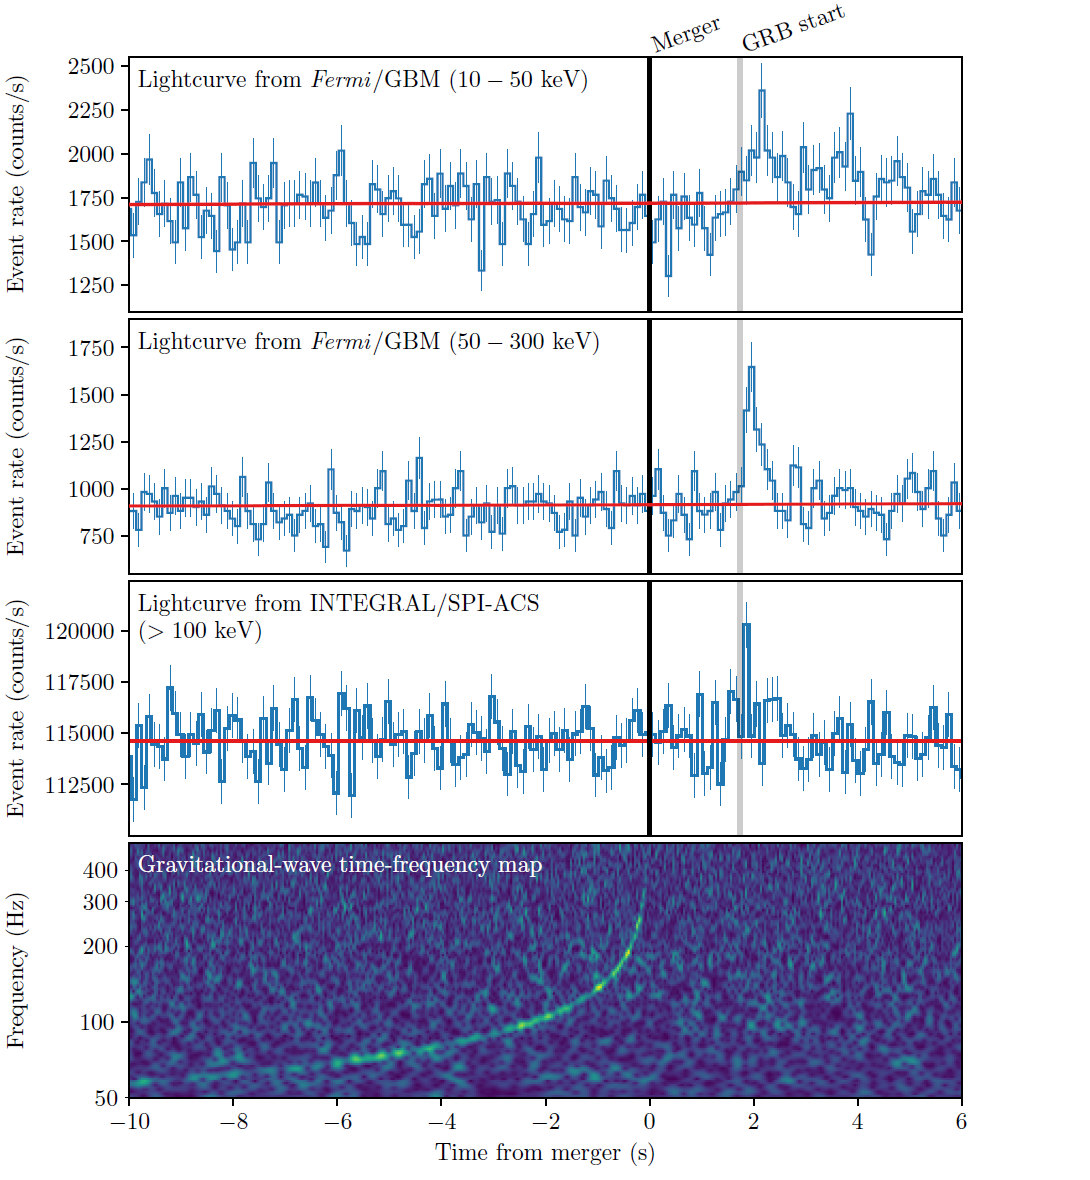
\includegraphics[keepaspectratio,height=14cm]{GW-GRB}\\
{\large [ApJ Let. 848 (2017) L13]}
\end{center}

\Tr
\twocolumn[\begin{center}{\blue Time spectrum analysis}\end{center}]
%
\begin{center}
{\red Possible source of time structure}\\[5mm]
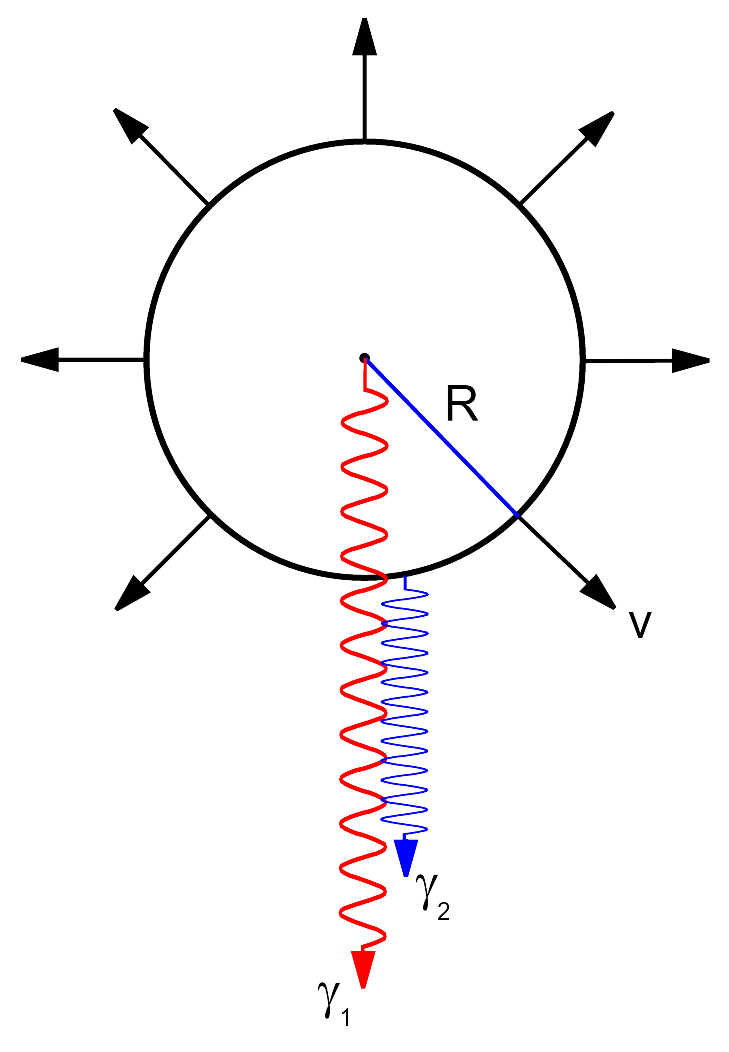
\includegraphics[keepaspectratio,height=10cm]{grb-shell3}
\end{center}
%
\begin{itemize}
\item If distance $r$ can be determined (see later)
\item[] $\rightarrow$ (Cosm.) time dilation correction known
\end{itemize}

\newpage

\begin{itemize}
\item Consider center of GRB as origin at rest
\item[] $\gamma_{1}$ produced at $t_{1}=0$
\item[] $\gamma_{2}$ produced at $t_{2}=t_{1}+R/v$
\item[] At some time $t>t_{2}$ we have
\item[] $r_{1}=ct$ and $r_{2}=R+c(t-R/v)$
\item $\gamma_{1}$ and $\gamma_{2}$ observed at the earth
\item[] $\displaystyle \Delta t=\frac{r_{1}-r_{2}}{c}=\frac{R}{c}\left(\frac{1}{\beta}-1\right)$
\item[] $\displaystyle \rightarrow \Delta t=\frac{R}{v}(1-\beta)
          \approx \frac{R}{v \gamma^{2}} \quad (\gamma \gg 1)$
\item[] {\blue Origin of the various spectral peaks~?}
\item Characteristic size $R$~?
\item[] Would allow determination of $\gamma$ factor
\end{itemize}

\Tr
\begin{center}
{\red Another source of time structure}
\end{center}

\vspace*{0.5cm}

\begin{itemize}
\item[] 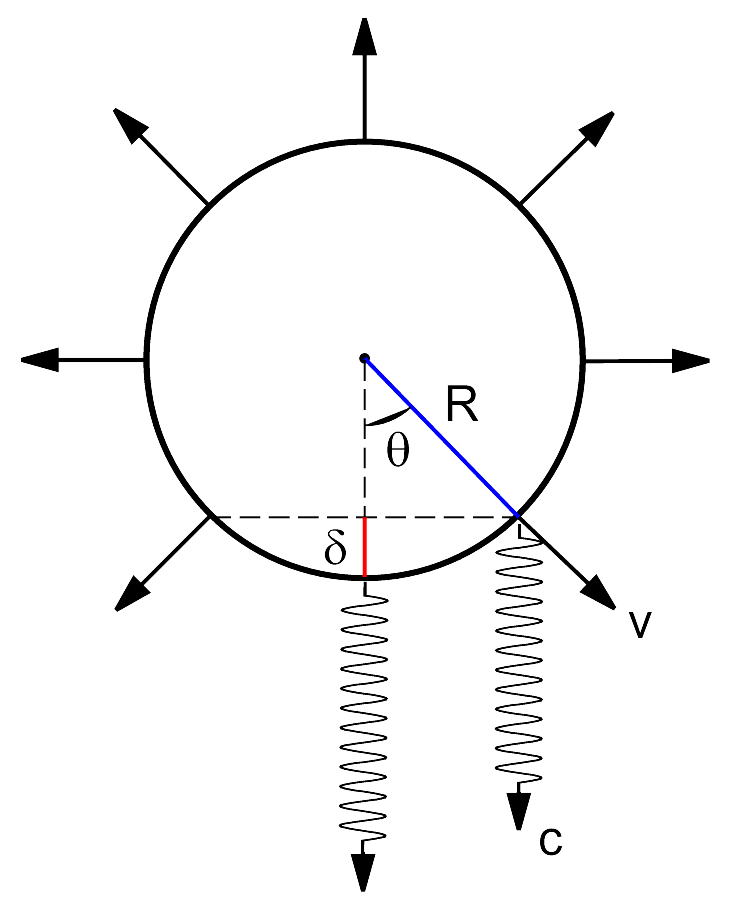
\includegraphics[keepaspectratio,height=7cm]{grb-shell1}
        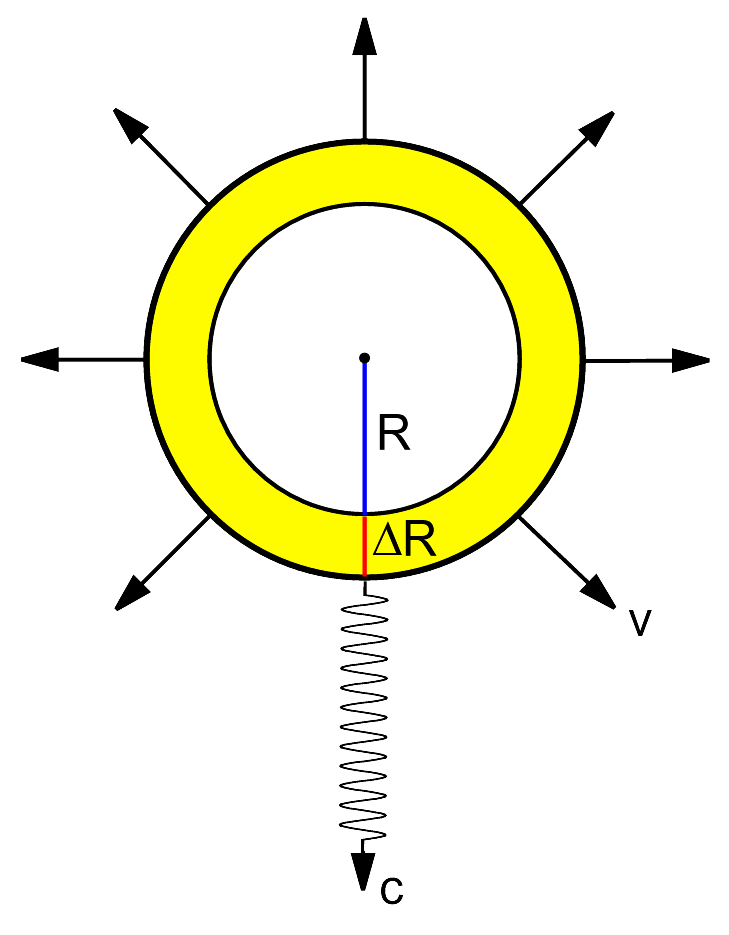
\includegraphics[keepaspectratio,height=7cm]{grb-shell2}
\item Observed duration $\Delta t \rightarrow R$ and $\Delta R$\\[2mm]
      $\displaystyle \Delta t=\frac{\delta}{c}=\frac{R}{c}\left(1-\cos\theta\right)$\\[2mm]
      $\rightarrow R=c\Delta t \quad$ Also : $\Delta R=c\Delta t$
\end{itemize}

\newpage

\vspace*{2.5cm}

\begin{itemize}
\item Quantities in CMS ($\ast$) via inverse Lorentz transformation of observables
\item[] Expanding shell $\rightarrow \gamma$
\item[] Cosmic expansion $\rightarrow \Gamma$
\item So we have ($\gamma \gg \Gamma$)
\item[] $\quad R^{\ast}=\Gamma R \qquad \Delta R^{\ast}=\gamma \Delta R$
\item[] $\quad E^{\ast}=\gamma^{-1} E$
\item {\blue Origin of the width of the peaks~?}
\end{itemize}

\Tr
\twocolumn[\begin{center}{\blue Burst location analysis}\end{center}]
%
\begin{center}
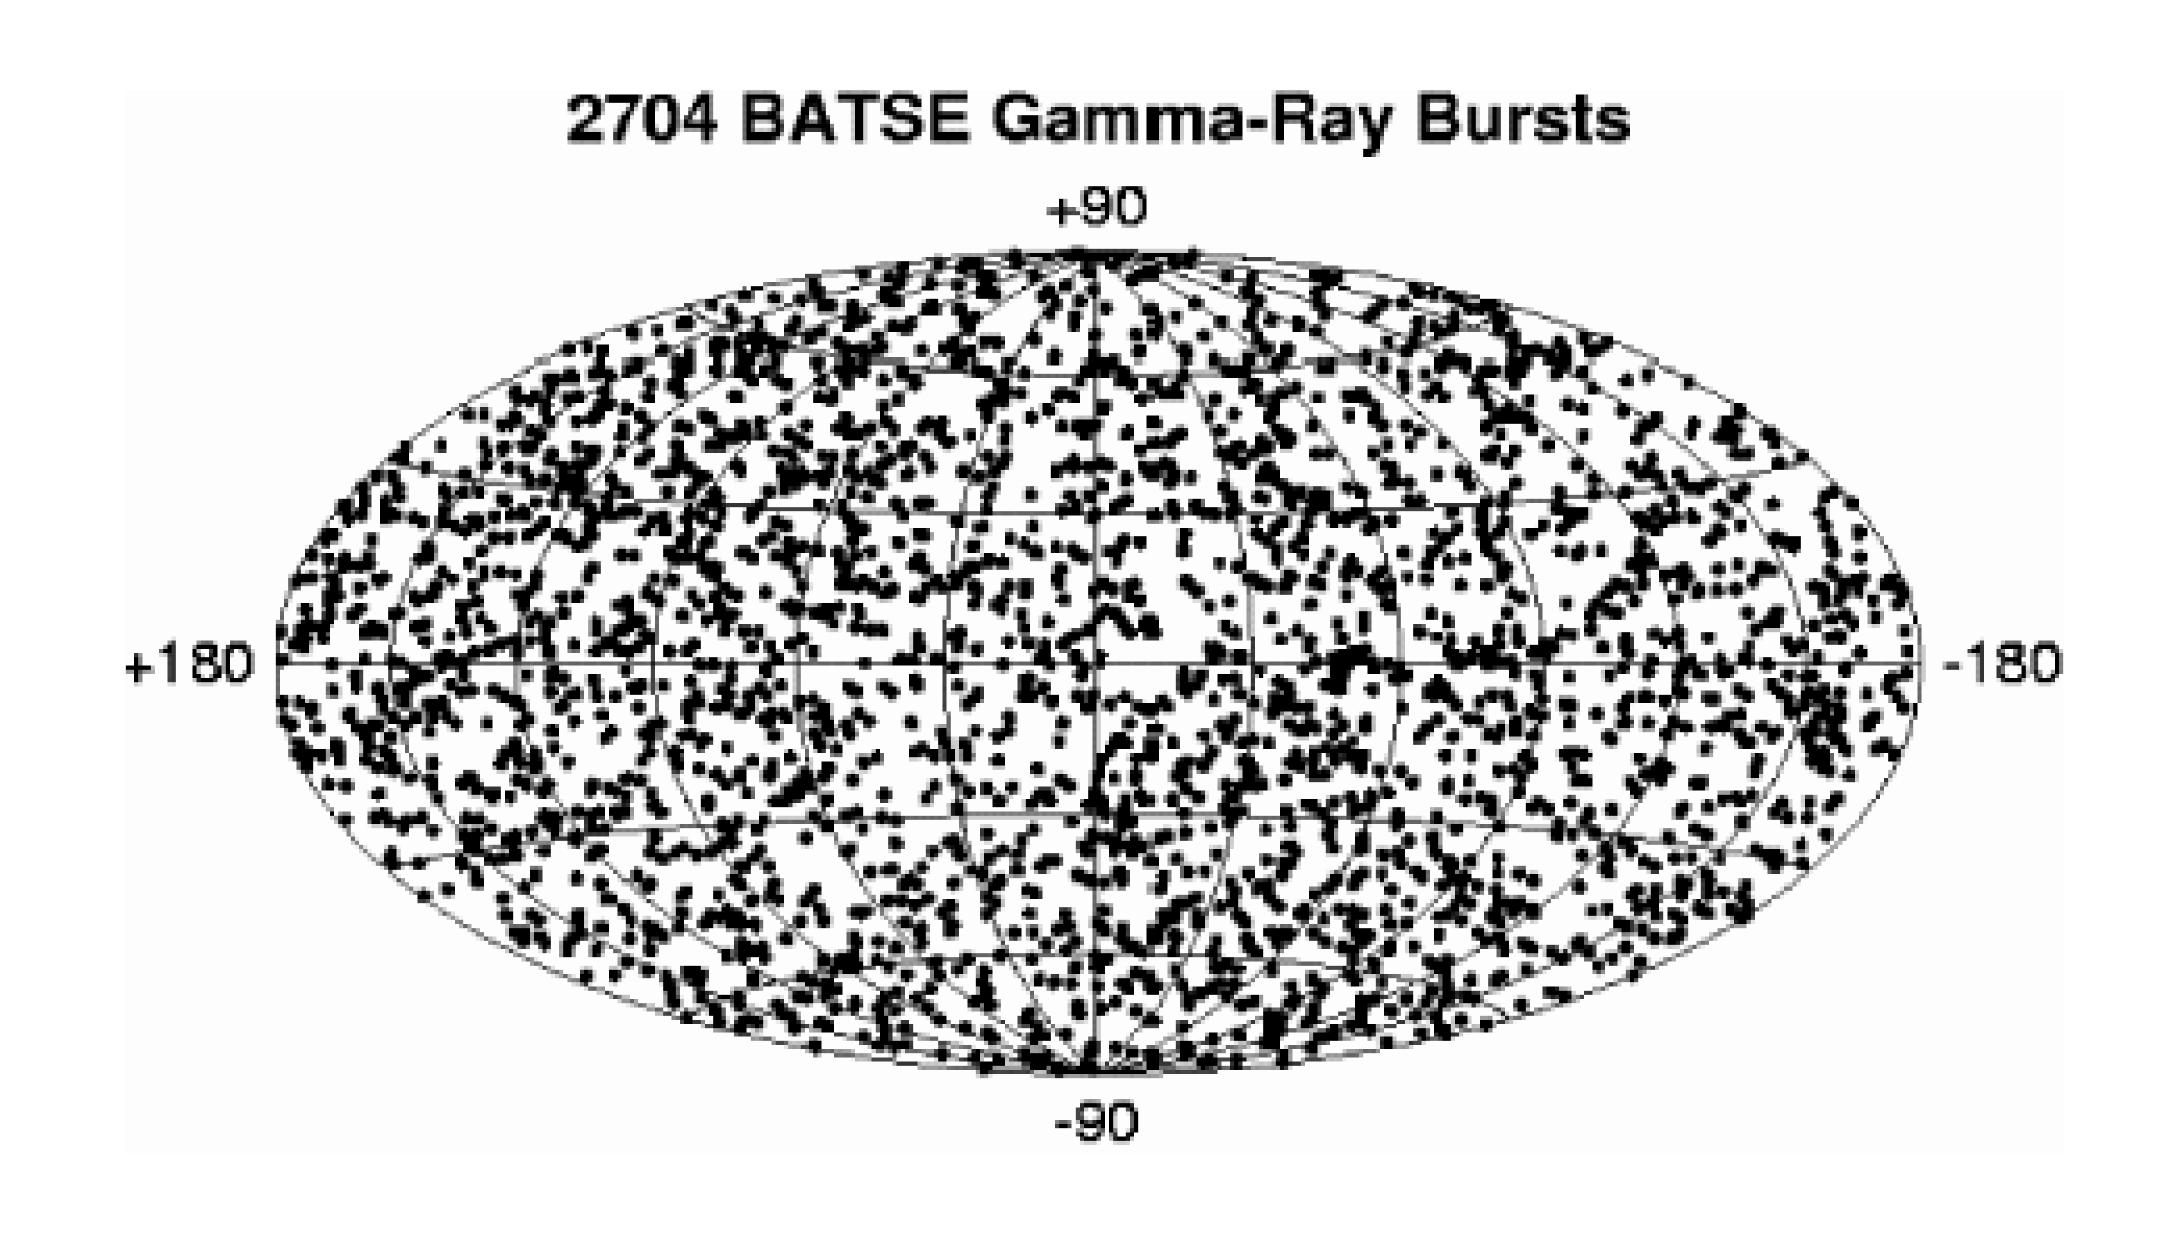
\includegraphics[keepaspectratio,width=13cm]{grbmap}
\end{center}
%
\begin{itemize}
\item No concentration along galactic plane
\item[] $\rightarrow$ Sources of cosmological origin
\item[] Confirmed by afterglow ($z$ values)
\item $(1+z)=\gamma(1+\beta) \quad$ (small $z$)
\item[] $\rightarrow \beta=\frac{(1+z)^{2}-1}{(1+z)^{2}+1}$ and $v=H_{0}r$
\end{itemize}
%
\begin{center}
{\red $z$ and Batse fluence yield total $E$}\\[3mm]
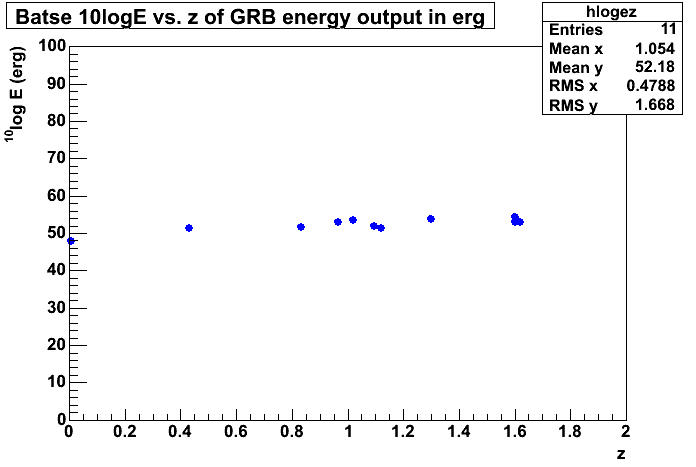
\includegraphics[keepaspectratio,width=13cm]{batse-loge-z}\\
No beaming and $H_{0}=71$ km/s Mpc$^{-1}$
\end{center}
%
\begin{itemize}
\item Characteristic energy output 
\item[] In Batse energy window $E_{0} \sim 10^{52}$ erg
\begin{itemize}
\item Allows to investigate distance distr.
\end{itemize}
\end{itemize}

\Tr
\begin{itemize}
\item Batse observed fluence $S$\\
      and assume $E_{0}$ for all bursts
\item[] $E_{0}=4\pi r^{2} S \rightarrow r=\left(\frac{E_{0}}{4\pi S}\right)^{1/2}$
\item[] \colorbox{yellow}{Batse data provide distance distribution}
\item $S=S_{0}$\\
      $\rightarrow$ specific distance $r_{0}=\left(\frac{E_{0}}{4\pi S_{0}}\right)^{1/2}$
\item[] Obviously $r < r_{0} \rightarrow S > S_{0}$
\item[] Homogeneous burst density $n$ Mpc$^{-1}$ yr$^{-1}$
\begin{itemize}
\item[] $\rightarrow N(>S_{0})=n\frac{4}{3}\pi r_{0}^{3} \propto S_{0}^{-3/2}$
\end{itemize}
\item[] \colorbox{yellow}{Batse data $N(>S_{0})$ vs. $S_{0}$ probe $n$}
\end{itemize}

\begin{itemize}
\item[$\ast$] {\blue Was there a specific GRB epoch~?}
\item[$\ast$] {\blue Match with cosmic-ray flux at the ankle~?}
\item[] Ankle~: $E^{2}\,\frac{\d N}{\d E} \approx 10^{-7}$ GeV cm$^{-2}$ s$^{-1}$
\end{itemize}

\newpage

\vspace*{1cm}

\begin{center}
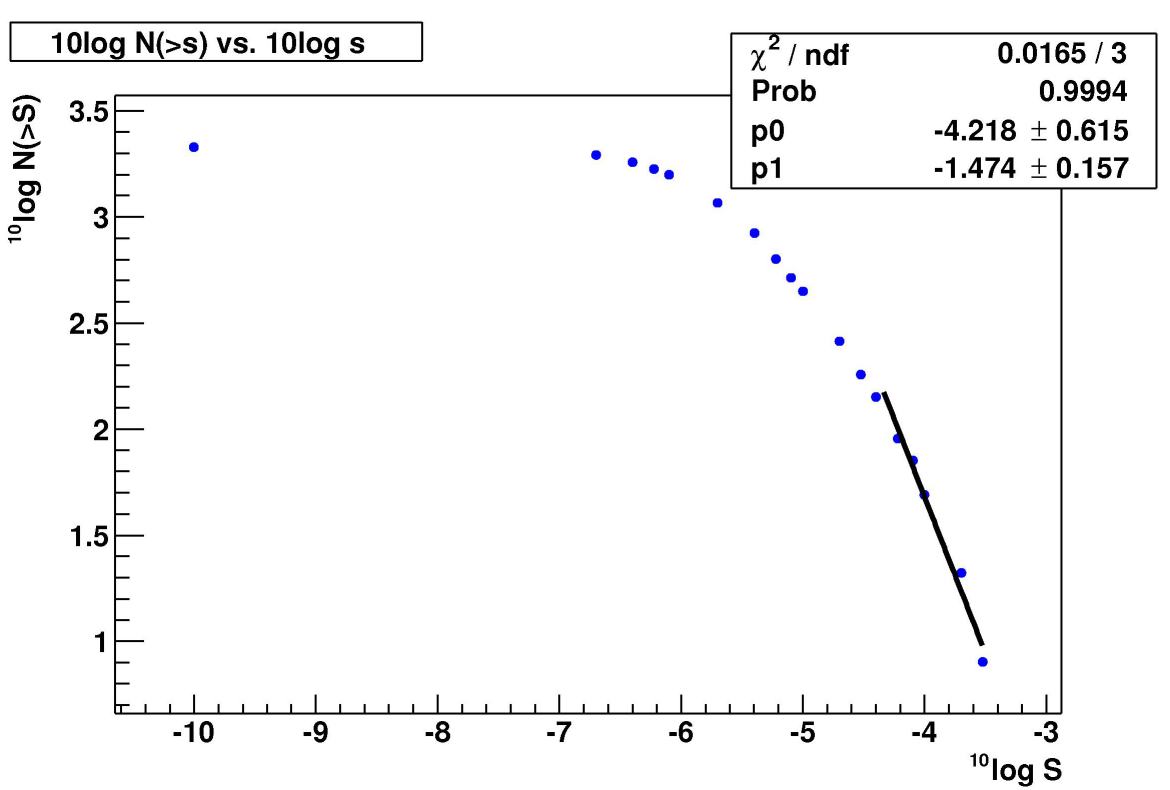
\includegraphics[keepaspectratio,width=13cm]{batse-n-s}
\end{center}
%
\begin{itemize}
{\red
\item Correction for redshift needed
\item Watch out for detector thresholds
}
\end{itemize}

\Tr
\onecolumn

\begin{itemize}
\item Using redshift and physical distance~:
      $\displaystyle S_{obs}=\frac{E_{0}}{4\pi (r_{phys})^{2}(1+z)}$\\[1mm]
\item Flat Friedmann-Lema\^{\i}tre universe and Robertson-Walker metric\\[1mm]
\item[] $\displaystyle r_{phys}(z_{obs})=\frac{c}{H_{0}}
        \int_{z=0}^{z=z_{obs}} \frac{\d z}{\sqrt{\Omega_{M}(1+z)^{3}+\Omega_{\Lambda}}}$\\[1mm]
\item[$\ast$] WMAP \& Planck observations (2013) : $\Omega_{M}=0.315 \pm 0.017 \quad \Omega_{\Lambda}=0.685 \pm 0.017$
\item[] $\rightarrow$ Integral needs to be solved numerically
\item[$\ast$] Simplified model~: $\Omega_{M}=1 \quad \Omega_{\Lambda}=0$
              $\displaystyle \rightarrow r_{phys}=\frac{2c}{H_{0}}\left( 1-\frac{1}{\sqrt{1+z}} \right)$\\[1mm]
\item $N(>S_{0})$ vs. $S_{0}$ analysis with simplified model yields~:
      $n=1.7 \cdot 10^{-10}$ Mpc$^{-3}$ yr$^{-1}$
\end{itemize}
